\documentclass[conference]{IEEEtran}
\usepackage[utf8]{inputenc}
\usepackage[T1]{fontenc}
\usepackage{graphicx}
\usepackage{amsmath,amssymb}
\usepackage{booktabs}
\usepackage{cite}
\usepackage{balance}
\usepackage{float}
\usepackage{dblfloatfix}
\usepackage{subcaption}

\begin{document}
\pagestyle{plain}

\title{MedVAE: Adaptation, Fine-tuning and Analysis for Medical Imaging and Coronary Segmentation}

\author{
\IEEEauthorblockN{Yanic Rothlingshofer \and Théo Palagi \and Elias Corlou \and Théophile Nadiedjoa}
}

\IEEEspecialpapernotice{\textit{\underline{Supervisor:} Elsa Angelini}}

\maketitle

\section{Introduction}

\section{Section 1: Théophile}

% ============================================================
\section{Robustesse de MedVAE aux dégradations d'entrée}
\label{sec:medvae-robustness}

MedVAE~\cite{varma2025medvae} est un autoencodeur perceptuel à grande
échelle conçu pour compresser des images médicales en représentations
latentes réduites tout en préservant les structures cliniquement
pertinentes lors de la reconstruction. Le modèle a été entraîné sur plus
d'un million d'images et évalué, dans son article d'origine, par PSNR et
MS-SSIM ainsi que par des études de lecteurs experts. Une question reste
toutefois ouverte pour un déploiement réel : \emph{comment la qualité de
reconstruction de MedVAE se comporte-t-elle lorsque l'image d'entrée
n'est pas propre, mais dégradée ?} En coronarographie, cette question est
loin d'être théorique : l'acquisition à faible dose induit un bruit
quantique important, et les images cliniques subissent compression, flou
de mouvement et artefacts variés~\cite{cesarelli2013xray}.

Nous évaluons cette robustesse sur le jeu de données
ARCADE~\cite{popov2023arcade}, constitué d'angiographies coronariennes
annotées. Le cadre est entièrement \emph{full-reference} : pour chaque
image nous disposons simultanément de l'image propre, d'une version
dégradée de façon contrôlée, et de la reconstruction produite par MedVAE
à partir de l'entrée dégradée. Cette configuration permet de tout
quantifier par comparaison directe, sans recourir à une métrique de
qualité sans référence. Plutôt que de chercher un unique axe de
« qualité d'entrée », nous distinguons deux mesures complémentaires :
l'écart entre l'image propre et l'image dégradée (l'amplitude de la
dégradation appliquée) d'une part, et la fidélité de la reconstruction
à son entrée dégradée d'autre part. La question de recherche devient
alors : \textbf{comment la fidélité de reconstruction de MedVAE
évolue-t-elle en fonction du type et de l'intensité de la dégradation
appliquée en entrée ?}

Nous montrons que la réponse dépend fortement de la \emph{nature} de la
dégradation, et non seulement de son intensité. En isolant trois types de
dégradation (bruit de Poisson, compression JPEG, flou gaussien), nous
mettons en évidence des régimes qualitativement distincts qui révèlent le
caractère passe-bas et débruiteur de MedVAE, ainsi que ses limites face
aux artefacts structurés.

% ============================================================
\subsection{Cadre d'évaluation}
\label{sec:cadre}

\subsubsection{Pourquoi écarter les métriques sans référence}
\label{sec:no-ref}

Une première approche, naturelle, consiste à quantifier la qualité de
l'image d'entrée par une métrique \emph{sans référence}, puis à la
corréler à la qualité de reconstruction. Nous avons exploré cette voie
avec ARNIQA~\cite{agnolucci2024arniqa}, ainsi qu'avec un score
sur mesure agrégeant des indices de netteté. Deux limites l'ont
disqualifiée. D'une part, ces métriques sont calibrées sur des photos
naturelles et transfèrent mal aux images de rayons X, où la notion de
« haute qualité perceptuelle » n'a pas le même sens : sur les images
brutes du jeu de données, la corrélation entre le score sans référence
et le PSNR de reconstruction est quasi nulle, la variance de qualité
intrinsèque entre images propres étant trop faible pour être exploitable.
D'autre part, sous dégradation contrôlée, ces scores sont dominés par le
flou et ne fournissent pas d'axe de qualité monotone, un biais cohérent
avec le fait que, dans l'espace de représentation d'ARNIQA, les
distorsions de flou ne forment pas de cluster
séparable~\cite{agnolucci2024arniqa}.

Or la difficulté est en réalité contournable : notre protocole est
intégralement \emph{full-reference}. Disposant de l'image propre, nous
n'avons pas besoin d'estimer la qualité d'entrée « à l'aveugle »,
nous pouvons la \emph{mesurer} directement par comparaison à la
référence. Nous abandonnons donc l'axe sans référence et redéfinissons
les deux quantités de l'étude de façon purement comparative :
\begin{itemize}
\itemsep0.2em
\item \textbf{Amplitude de dégradation} : $\mathrm{PSNR}(\text{propre},
      \text{dégradée})$, qui mesure de combien l'entrée s'écarte de
      l'image propre ;
\item \textbf{Fidélité de reconstruction} : $\mathrm{PSNR}(\text{dégradée},
      \text{reconstruite})$, qui mesure la fidélité de MedVAE à l'entrée
      qu'on lui présente.
\end{itemize}
Ces deux mesures répondent à des questions distinctes et ne doivent pas
être confondues : la seconde caractérise le comportement du modèle, la
première sert uniquement d'abscisse contrôlée.

\subsubsection{PSNR masqué sur les vaisseaux}
\label{sec:masked-psnr}

Un PSNR calculé sur l'image entière est trompeur en coronarographie : le
fond occupe la très grande majorité de la surface, si bien qu'un PSNR
global reflète surtout la fidélité du fond et non celle des vaisseaux,
la seule région cliniquement pertinente. Ce biais est tel que le PSNR
global peut \emph{augmenter} lorsque l'image se dégrade, le fond lissé
devenant plus « facile » à reproduire. Nous restreignons donc le calcul
aux pixels de vaisseaux, obtenus en rastérisant les annotations
polygonales d'ARCADE (format COCO) en masque binaire, ce qui définit un
PSNR masqué noté $\mathrm{mPSNR}$. Les deux mesures ci-dessus (amplitude
de dégradation et fidélité de reconstruction) sont calculées dans cette
version masquée. Le détail du calcul, l'équation et une illustration sur
un exemple réel sont donnés en annexe~\ref{app:mpsnr}.

% ============================================================
\subsection{Méthode}
\label{sec:methode}

\subsubsection{Protocole}
\label{sec:protocole}

Nous utilisons l'autoencodeur \texttt{medvae\_4\_1\_2d} (modalité rayons
X), appliqué aux angiographies du sous-ensemble de segmentation d'ARCADE.
Le prétraitement est celui fourni par MedVAE (\texttt{apply\_transform}).
Pour chaque type de dégradation, le protocole est le suivant : on tire
aléatoirement $50$ images propres parmi les $1000$ disponibles (tirage
sans remise, graine fixée pour la reproductibilité), puis on applique une
rampe linéaire de $20$ niveaux d'intensité croissante. À chaque niveau et
pour chaque image, on calcule les deux mesures masquées
$\mathrm{mPSNR}(\text{propre}, \text{dégradée})$ et
$\mathrm{mPSNR}(\text{dégradée}, \text{reconstruite})$, moyennées sur les
$50$ images. Le masque de vaisseaux est commun aux deux mesures pour une
image donnée. L'inférence MedVAE est intégrée à la boucle de sweep, ce qui
produit la reconstruction de chaque entrée dégradée. Les effectifs
volontairement modestes ($50$ images, $20$ niveaux) sont contraints par la
puissance de calcul disponible.

% ---------- Figure pleine largeur : pipeline ----------
\begin{figure*}[t]
  \centering
  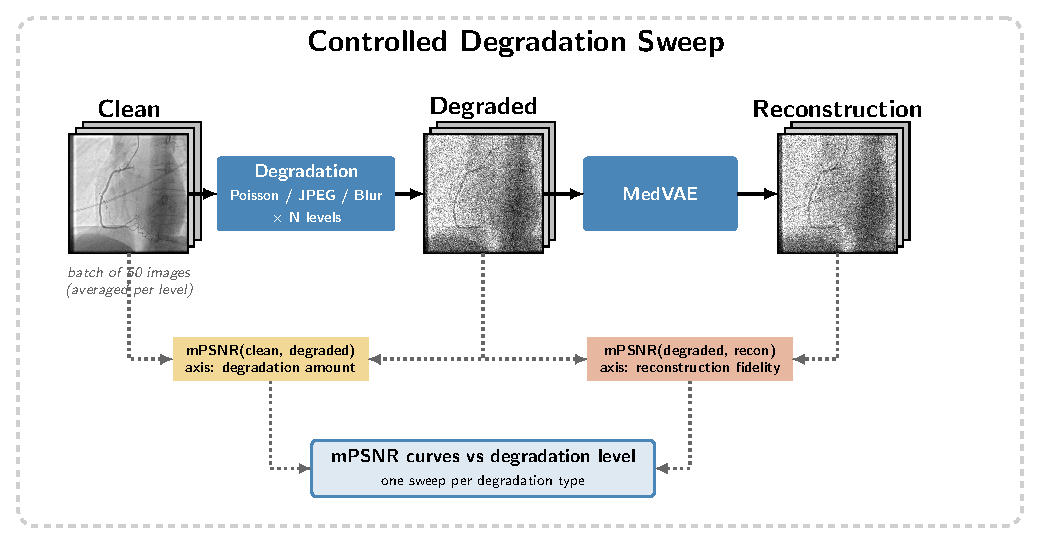
\includegraphics[width=0.92\textwidth]{figures/elias/pipeline.pdf}
  \caption{Pipeline d'évaluation. Un batch d'images propres est dégradé de
  façon contrôlée sur $N$ niveaux, puis reconstruit par MedVAE. Deux
  mesures masquées (vessel-only) sont calculées par niveau et moyennées sur
  le batch : $\mathrm{mPSNR}(\text{propre}, \text{dégradée})$ quantifie
  l'amplitude de la dégradation appliquée, et
  $\mathrm{mPSNR}(\text{dégradée}, \text{recon})$ la fidélité de
  reconstruction. Un sweep distinct est mené par type de dégradation
  (Poisson, JPEG, flou).}
  \label{fig:pipeline}
\end{figure*}

\subsubsection{Sweeps séparés par type de dégradation}
\label{sec:sweeps-separes}

Conformément à l'analyse précédente, qui montrait qu'une rampe combinant
plusieurs dégradations rend l'interprétation impossible, le flou
écrasant les autres effets, nous menons \emph{un sweep distinct par
type de dégradation}. Cela isole l'effet propre de chaque perturbation sur
la reconstruction.

\subsection{Types de dégradation}
\label{sec:degradations}

Trois dégradations sont étudiées, chacune balayée seule :

\textbf{Bruit de Poisson.} Plus réaliste que le bruit gaussien pour les
rayons X, où le bruit quantique (\emph{shot noise}) domine à faible
dose~\cite{cesarelli2013xray}. L'intensité est pilotée par un facteur
d'échelle décroissant : plus l'échelle diminue, moins de photons sont
simulés et plus le bruit est marqué.

\textbf{Compression JPEG.} Facteur de qualité décroissant de $95$ à $5$,
qui introduit successivement la quantification des coefficients DCT puis
les artefacts de blocs $8\times8$.

\textbf{Flou gaussien.} Taille de noyau croissante (noyaux forcés impairs).
Le niveau le plus bas, de noyau unitaire, correspond à l'image propre.

\section{Résultats et interprétation}
\label{sec:resultats}

Pour chaque type de dégradation, nous traçons l'évolution des métriques en fonction du niveau d'intensité (figure~\ref{fig:sweep-all}). La courbe \emph{amplitude de dégradation}, $\mathrm{mPSNR}(\text{propre}, \text{dégradée})$, décroît par construction et sert d'abscisse contrôlée. La courbe d'intérêt est la \emph{fidélité de reconstruction}, $\mathrm{mPSNR}(\text{dégradée}, \text{reconstruite})$, qui caractérise le comportement de MedVAE. Une troisième courbe, $\mathrm{mPSNR}(\text{propre}, \text{reconstruite})$, n'est tracée que pour le bruit de Poisson, où elle teste l'hypothèse de débruitage (section~\ref{sec:poisson}).

La conclusion d'ensemble est que la réponse de MedVAE ne dépend pas seulement de l'intensité de la dégradation mais de sa \emph{nature spectrale} : selon que la perturbation retire ou ajoute des hautes fréquences, et selon que ces hautes fréquences sont structurées ou non, la fidélité de reconstruction varie dans des directions opposées. Ce comportement est cohérent avec le biais spectral des réseaux de neurones~\cite{rahaman2019spectral} et avec le caractère passe-bas connu des autoencodeurs. Les valeurs de corrélations associées à ces observations sont synthétisées dans la table~\ref{tab:stats-correlation}.

% ---------- Figure globale sur deux colonnes ----------
\begin{figure*}[t]
  \centering
  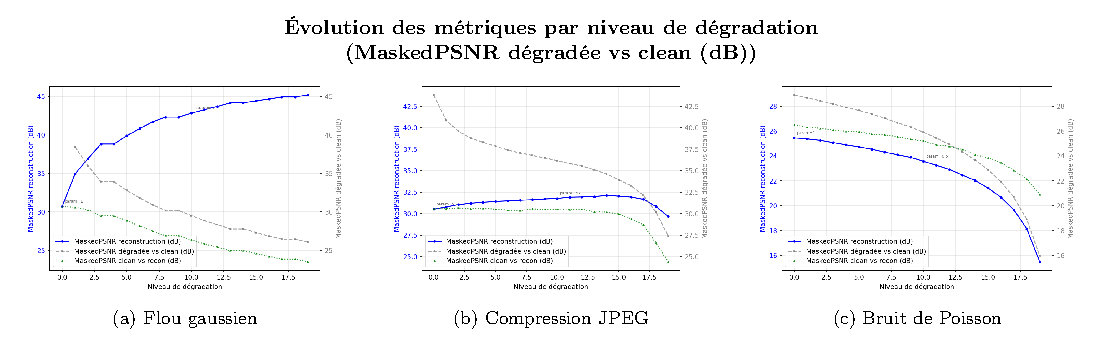
\includegraphics[width=\linewidth]{figures/elias/metrics_by_level_all_masked.pdf}
  \caption{Évolution des métriques mPSNR pour le bruit de Poisson, la compression JPEG et le flou gaussien. La fidélité de reconstruction (bleu) réagit différemment selon la nature de la dégradation.}
  \label{fig:sweep-all}
\end{figure*}

% ---------- Tableau des statistiques ----------
\begin{table}[h]
\centering
\footnotesize
\setlength{\tabcolsep}{4pt}
\caption{Corrélations entre fidélité de reconstruction et amplitude de dégradation ($r$ : Pearson, $\rho$ : Spearman).}
\label{tab:stats-correlation}
\begin{tabular}{@{}llrrr@{}}
\toprule
Dégradation & Régime & $r$ & $\rho$ & $p$-value \\
\midrule
Flou & Global & $-0{,}998$ & $-0{,}998$ & $< 10^{-4}$ \\
Poisson & Global & $+0{,}998$ & $+1{,}000$ & $< 10^{-4}$ \\
\midrule
JPEG & Global & $+0{,}030$ & $-0{,}439$ & $0{,}90$ \\
     & Avant pic & $-0{,}990$ & $-1{,}000$ & $< 10^{-4}$ \\
     & Après pic & $+0{,}990$ & $+1{,}000$ & $< 10^{-4}$ \\
\bottomrule
\end{tabular}
\end{table}

\subsubsection{Flou gaussien : anti-corrélation}
\label{sec:flou}

Résultat le plus marquant : quand l'entrée se dégrade, la reconstruction \emph{s'améliore}, passant d'environ $28{,}9$ à $39{,}2$~dB. Les deux courbes sont quasi symétriques, et la corrélation entre fidélité et amplitude de dégradation est très fortement négative (cf. table~\ref{tab:stats-correlation}), avec une pente de régression de $-0{,}84$~dB par dB de dégradation.

L'explication tient au caractère passe-bas des autoencodeurs. Un VAE compresse vers un espace latent de faible dimension : il reproduit fidèlement les basses fréquences mais mal les hautes, un phénomène désigné sous le terme de biais spectral, les réseaux apprenant préférentiellement les composantes basse fréquence d'un signal~\cite{rahaman2019spectral}. Une image floutée vit déjà essentiellement dans ce sous-espace basse fréquence que MedVAE reproduit bien : elle est « facile » à reconstruire. Ce que le flou retire à l'entrée, il le rend simultanément facile à reconstruire, d'où la symétrie observée. Ce résultat confirme de façon propre et monotone le rôle particulier du flou, qui motivait l'abandon des métriques sans référence.

\subsubsection{Bruit de Poisson : corrélation positive et débruitage}
\label{sec:poisson}

Comportement miroir du flou, et attendu : le bruit de Poisson ajoute des hautes fréquences décorrélées, précisément ce que le latent n'encode pas. L'entrée s'éloigne du propre et la reconstruction se dégrade en parallèle, les deux courbes étant quasi confondues. La corrélation est très fortement positive et la fidélité de reconstruction chute de $19{,}5$ à $9{,}5$~dB sur le sweep.

Le mécanisme sous-jacent est celui du débruitage par autoencodeur : le goulot latent ne peut pas représenter le bruit haute fréquence, donc il le supprime~\cite{vincent2008denoising}. Nous le vérifions directement grâce à la troisième courbe : sur l'intégralité du sweep ($100\%$ des niveaux), la reconstruction est plus proche de l'image \emph{propre} que de l'image \emph{dégradée} qui lui a été présentée en entrée, soit $\mathrm{mPSNR}(\text{propre}, \text{reconstruite}) > \mathrm{mPSNR}(\text{dégradée}, \text{reconstruite})$, avec un écart moyen de $+1{,}94$~dB. La sortie de MedVAE pointe donc vers le signal et non vers le bruit : le débruitage est réel et directionnel.

Cette restauration reste toutefois partielle. Comparée non plus à l'entrée mais à l'amplitude de dégradation, $\mathrm{mPSNR}(\text{propre}, \text{reconstruite})$ demeure \emph{en deçà} de $\mathrm{mPSNR}(\text{propre}, \text{dégradée})$ sur les pixels de vaisseaux : passer par MedVAE ne rapproche pas l'image du propre davantage que ne le ferait l'entrée bruitée laissée telle quelle. L'erreur de reconstruction intrinsèque du modèle, liée à la compression latente avec perte, l'emporte sur le gain de débruitage dans la région cliniquement pertinente. Autrement dit, MedVAE débruite dans la bonne direction, mais ce débruitage ne suffit pas à restaurer une image diagnostiquement fidèle.

\subsubsection{Compression JPEG : deux régimes}
\label{sec:jpeg}

La compression JPEG produit une réponse \emph{non monotone} : la fidélité de reconstruction monte d'abord légèrement jusqu'au niveau~$14$ (pic à environ $26$~dB), puis s'effondre. Cette non-monotonie a une conséquence statistique directe : un coefficient de corrélation calculé sur l'ensemble du sweep est trompeur. C'est une illustration du fait que les coefficients de corrélation globaux (Pearson pour la linéarité, Spearman pour la monotonie) sont aveugles aux relations non monotones et masquent ici une dynamique en deux régimes. En séparant au pic, chaque régime est au contraire presque parfaitement corrélé (table~\ref{tab:stats-correlation}).

Ces deux régimes correspondent à deux comportements physiques distincts. En haute et moyenne qualité, JPEG quantifie les coefficients DCT et supprime les hautes fréquences : il agit comme un passe-bas par blocs, se comporte comme le flou et rend l'entrée plus « compatible » avec le latent de MedVAE, d'où la légère hausse de fidélité. En basse qualité apparaissent les artefacts de blocs $8\times8$ et le \emph{ringing} autour des contours, des structures hautes fréquences \emph{spatialement organisées} et absentes des données d'entraînement. MedVAE ne sait ni les encoder ni les ignorer proprement, d'où l'effondrement de la reconstruction. JPEG combine ainsi les deux mécanismes précédents : le régime « flou » qui aide, puis le régime « bruit structuré » qui casse la reconstruction.

\subsection{Discussion et ouvertures}
\label{sec:discussion}

L'étude croisée de ces trois perturbations met en lumière la mécanique interne de MedVAE. Le modèle agit fondamentalement comme un filtre passe-bas intelligent et un débruiteur non linéaire : il est optimisé pour reproduire fidèlement les basses fréquences (flou gaussien) et rejeter les hautes fréquences stochastiques (bruit de Poisson). Sa limite majeure réside toutefois dans sa vulnérabilité aux hautes fréquences \emph{structurées} hors distribution (artefacts JPEG), qu'il ne parvient ni à ignorer ni à reconstruire, corrompant ainsi l'image de sortie.

Ces caractéristiques appellent plusieurs perspectives d'évaluation clinique. En premier lieu, il conviendra de quantifier l'impact de cette dynamique passe-bas sur la détection des sténoses, tâche centrale du jeu de données ARCADE, ces pathologies constituant des structures fines particulièrement sensibles au lissage. Par ailleurs, l'exploration de l'espace latent (détaillée en section ??) révèle que MedVAE encode massivement les gradients de luminosité et de contraste. Évaluer sa robustesse face à des altérations de la dynamique des niveaux de gris (variations gamma, sous-exposition) constitue donc une prochaine étape naturelle. Enfin, le protocole gagnerait à intégrer le flou de mouvement : induit par les dynamiques cardiaques et respiratoires~\cite{topol1995luminology}, ce flou directionnel constitue un artefact clinique omniprésent en coronarographie, dont la signature spectrale est bien plus complexe que le flou isotrope modélisé ici.

% ============================================================
\newpage
\section{JEPA Adaptation of MedVAE Stage 2}

MedVAE~\cite{varma2025medvaeefficientautomatedinterpretation} is a generalised variational autoencoder (VAE) for medical imaging, trained in two stages: the first learns faithful reconstruction, the second enriches the latent space with semantic knowledge. Medical imaging raises specific challenges — monochrome images, scarce annotations, heterogeneous modalities — that make learning robust representations particularly difficult.

\subsection{Motivations}

In its original formulation, MedVAE stage 2 aligns the latent space with BioMedCLIP representations, a foundation model pre-trained on paired medical image–text corpora. This approach has two structural limitations. First, it requires paired image–text data at inference time, which is unavailable for many clinical workflows. Second, and more fundamentally, the alignment inherits BioMedCLIP's biases and coverage gaps: coronary angiography represents a narrow and specialised sub-domain in large-scale medical vision–language pretraining, so the transmitted semantic signal may be weak or misleading. Aligning to a model that has never seen enough coronary images is unlikely to produce representations that are discriminative for vascular anatomy.

JEPA (\textit{Joint-Embedding Predictive Architecture}) architectures~\cite{assran2023selfsupervisedlearningimagesjointembedding} offer a self-supervised alternative that removes the dependency on any external model. Rather than reconstructing masked pixels — which can waste capacity on low-level texture — JEPA predicts in latent space the representations of masked regions. This forces the encoder to model the contextual relationships between visible patches and occluded areas, learning representations that are inherently structured and high-level. The approach has shown strong results across medical imaging modalities: US-JEPA~\cite{radhachandran2026usjepajointembeddingpredictive} for ultrasound, EchoJEPA~\cite{munim2026echojepalatentpredictivefoundation} for echocardiography, Brain-JEPA~\cite{NEURIPS2024_9c3828ad} for fMRI, and Seg-JEPA~\cite{10.1007/978-981-92-0068-9_7} for segmentation.

We propose replacing stage 2's BioMedCLIP alignment with JEPA training directly on coronary angiography images, with no dependency on an external model. The stage-1 encoder and decoder weights are kept as initialisation and the decoder remains frozen throughout, so any gain in latent structure can be evaluated independently of reconstruction quality.

\subsection{Method}

\paragraph{Original stage 2 — BioMedCLIP alignment.}
In the original MedVAE formulation (Fig.~\ref{fig:stage2ori}), stage 2 fine-tunes the encoder by minimising the distance between the VAE's latent representations and BioMedCLIP embeddings for the same images. This step aims to semantically enrich the latent space by transmitting the knowledge of a pre-trained medical foundation model.

\begin{figure}[htbp]
    \centering
    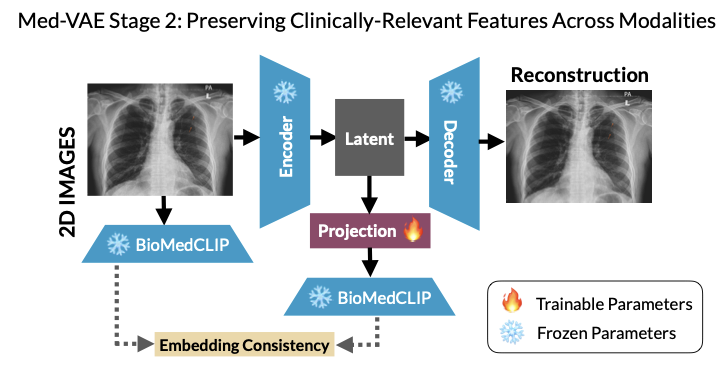
\includegraphics[width=\columnwidth]{figures/yanic/stage_2_medvae_ori.png}
    \caption{Original stage 2: latent space alignment on BioMedCLIP embeddings.}
    \label{fig:stage2ori}
\end{figure}

\paragraph{Modified stage 2 — JEPA adaptation.}
We replace the BioMedCLIP alignment with JEPA training directly on coronary angiography images (Fig.~\ref{fig:stage2}). The architecture has three components, all operating in the stage-1 VAE latent space:

\begin{itemize}
    \item \textbf{Context encoder}: the stage-1 encoder (frozen decoder), receiving the masked image (40\% of patches zeroed) and producing the context latent $z_c$.
    \item \textbf{Target encoder}: EMA copy of the context encoder with \texttt{stop-gradient}, encoding the full image. Weights updated as $\theta_t \leftarrow m\,\theta_t + (1-m)\,\theta_c$ ($m = 0{.}996$).
    \item \textbf{JEPA predictor}: lightweight convolutional network (depth 3, hidden dim 128) taking $z_c$ concatenated with a binary mask of target patches, predicting $\hat{z}_t$.
\end{itemize}

\begin{figure}[htbp]
    \centering
    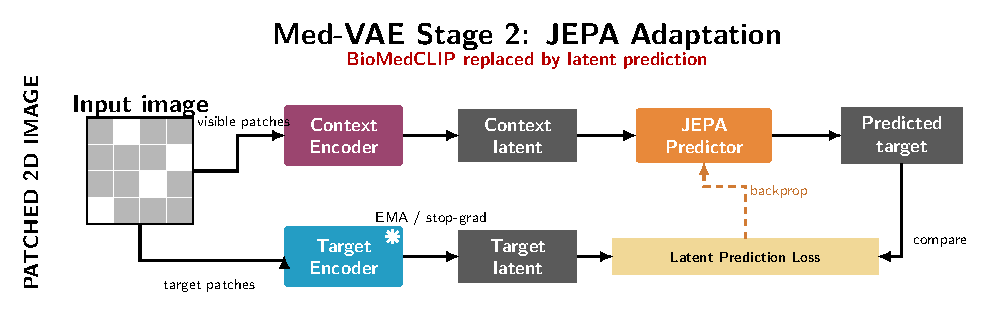
\includegraphics[width=\columnwidth]{figures/yanic/stage_2_pipeline.pdf}
    \caption{Modified stage 2: JEPA adaptation — the context encoder predicts the target latent of the EMA encoder (stop-grad).}
    \label{fig:stage2}
\end{figure}

\paragraph{Loss function.}
The stage-2 loss is:
\begin{equation}
    \mathcal{L}_{\text{stage2}} = \mathcal{L}_{\text{pred}} + \lambda_{\text{SIGReg}} \, \mathcal{L}_{\text{SIGReg}},
    \label{eq:stage2}
\end{equation}
where $\mathcal{L}_{\text{pred}}$ is the Smooth-$L_1$ loss between $\hat{z}_t$ and the channel-wise normalised target latent $\tilde{z}_t$, restricted to masked patches $\mathcal{M}$:
\begin{equation}
    \mathcal{L}_{\text{pred}} = \frac{1}{|\mathcal{M}|} \sum_{p \in \mathcal{M}} \mathrm{SmoothL_1}\!\left(\hat{z}_t^{(p)},\; \tilde{z}_t^{(p)}\right),
\end{equation}
and $\mathcal{L}_{\text{SIGReg}}$ is the SIGReg regularisation~\cite{balestriero2025lejepaprovablescalableselfsupervised} on $z_c$, based on the Epps–Pulley statistic applied to random projections of the embeddings:
\begin{equation}
    \mathcal{L}_{\text{SIGReg}} = \mathbb{E}_{\mathbf{v}}\!\left[ T_{\text{EP}}\!\left(\bigl\{ z_c^\top \mathbf{v} \bigr\}\right) \right].
\end{equation}
This term prevents representational collapse without negative pairs. In practice $\lambda_{\text{SIGReg}} = 0{.}01$.

\paragraph{Collapse risks.}
JEPA training is exposed to three degenerate modes. \textbf{Representational collapse} occurs when the encoder produces a constant representation that the predictor learns to imitate — normalising $\tilde{z}_t$ channel-wise makes this solution explicitly penalised. \textbf{Dimensional collapse} corresponds to the progressive extinction of certain latent dimensions; $\mathcal{L}_{\text{SIGReg}}$ detects and corrects this by maintaining an isotropic distribution over random projections. Finally, a \textbf{too-low EMA momentum} would cause the target encoder to converge too quickly towards the context encoder, cancelling the learning signal — hence the choice of $m = 0{.}996$, which keeps the target encoder as a slow-moving average.

At the end of stage 2, one expects a latent space where patches that are anatomically similar produce nearby representations regardless of their spatial position. The predictor acts as a local world model: inferring a masked patch requires understanding the global structure of the image, which forces the encoder to acquire semantically informative representations rather than encoding low-level intensity patterns.

\subsection{Results}

\paragraph{Reconstruction quality.}
During stage 2 the decoder remains frozen, so any displacement of the encoder into a subspace incompatible with the decoder directly degrades reconstruction. Table~\ref{tab:recon} reports metrics on 100 ARCADE validation images; Fig.~\ref{fig:recon} illustrates the effect on a representative image.

\begin{table}[htbp]
\centering\small
\begin{tabular}{@{}lccc@{}}
\toprule
Model & MSE ($\!\times\!10^{-3}$) & MAE & PSNR (dB) \\
\midrule
MedVAE orig. & 2.23 & 0.033 & 32.54 \\
Stage 1      & 3.32 & 0.041 & 30.81 \\
Stage 2 JEPA & 82.7 & 0.230 & 16.85 \\
\bottomrule
\end{tabular}
\caption{Reconstruction on 100 ARCADE images (range $[-1,1]$).}
\label{tab:recon}
\end{table}

\begin{figure}[htbp]
    \centering
    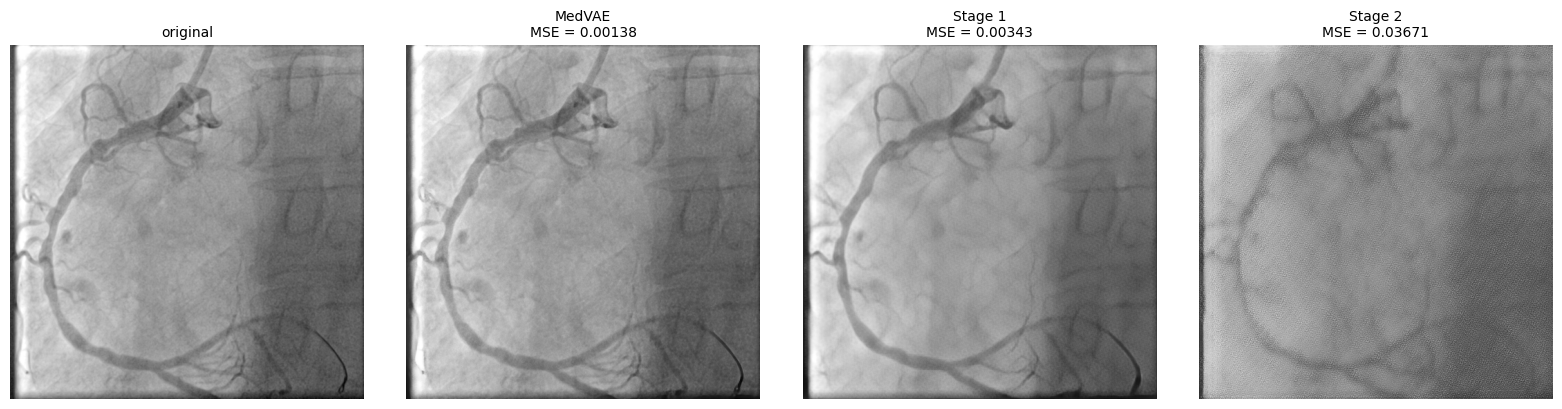
\includegraphics[width=\columnwidth]{figures/yanic/recon.png}
    \caption{Reconstruction on an ARCADE image: original, MedVAE, Stage 1, Stage 2 (left to right).}
    \label{fig:recon}
\end{figure}

\paragraph{Latent space structure.}
We measure the effective dimensionality via effective rank $\rho = \exp\!\bigl(-\sum_i \bar\sigma_i \log \bar\sigma_i\bigr)$, and vascular class separability via KNN-5 and a linear probe on 300 annotated ARCADE images.

\begin{table}[htbp]
\centering
\resizebox{\columnwidth}{!}{\begin{tabular}{@{}lcccc@{}}
\toprule
Model & Eff. rank & Dims@90\% & KNN-5 & Lin. probe \\
\midrule
MedVAE orig. & 256.6 & 200         & 18.3\,\% & 15.0\,\% \\
Stage 1      & 239.5 & 161         & 21.7\,\% & 25.0\,\% \\
Stage 2 JEPA & 164.0 & \textbf{25} & 18.3\,\% & 21.7\,\% \\
\bottomrule
\end{tabular}}
\caption{Latent structure and vascular separability. Dims@90\% = number of PCA components for 90\% of variance.}
\label{tab:latent}
\end{table}

The effective rank decreases at each stage: $256.6 \to 239.5 \to 164.0$. The most striking finding is the number of active dimensions: stage 2 concentrates 90\% of its variance on only \textbf{25 dimensions} (vs. 161 for stage 1 and 200 for the original). This is characteristic of JEPA architectures — the patch-prediction objective selects a restricted but coherent subspace — and occurs without total collapse, since the effective rank remains at 164. The linear probe confirms that ARCADE adaptations bring discriminative gain over the original model (stage 1: 25.0\%, stage 2: 21.7\%, original: 15.0\%). The slight drop from stage 1 to stage 2 suggests a trade-off: JEPA's global contextual objective produces more concentrated representations that are slightly less linearly separable than the stage-1 features, while still outperforming the unspecialised baseline.

\paragraph{Intermediate feature visualisation — RGB PCA.}
To go beyond the limitations of the 1-channel bottleneck, we analyse the feature maps of the last residual block before \texttt{conv\_out} (256 channels, $64{\times}64$ resolution). We apply PCA with 3 components across these spatial vectors: PC1$\to$R, PC2$\to$G, PC3$\to$B, with percentile normalisation [2\%, 98\%], following the visualisation protocol of DINO~\cite{caron2021emergingpropertiesselfsupervisedvision} and LeJEPA~\cite{balestriero2025lejepaprovablescalableselfsupervised}. Fig.~\ref{fig:pca} reveals three distinct behaviours. The original MedVAE exhibits a pronounced border artefact — a coloured frame delimiting the image interior, reflecting a generalised pretraining that attends to image boundaries. Stage 1 produces the most spatially coherent features: the vascular trace emerges in a distinct hue from the background, suggesting that fine-tuning on ARCADE already concentrates discriminative information along the coronary tree. Stage 2 JEPA generates near-uniform large-scale features, which may seem counterintuitive but is consistent with the dimensional contraction observed in Table~\ref{tab:latent}: the patch-prediction objective favours a global contextual representation rather than a fine-grained local one.

\begin{figure}[htbp]
    \centering
    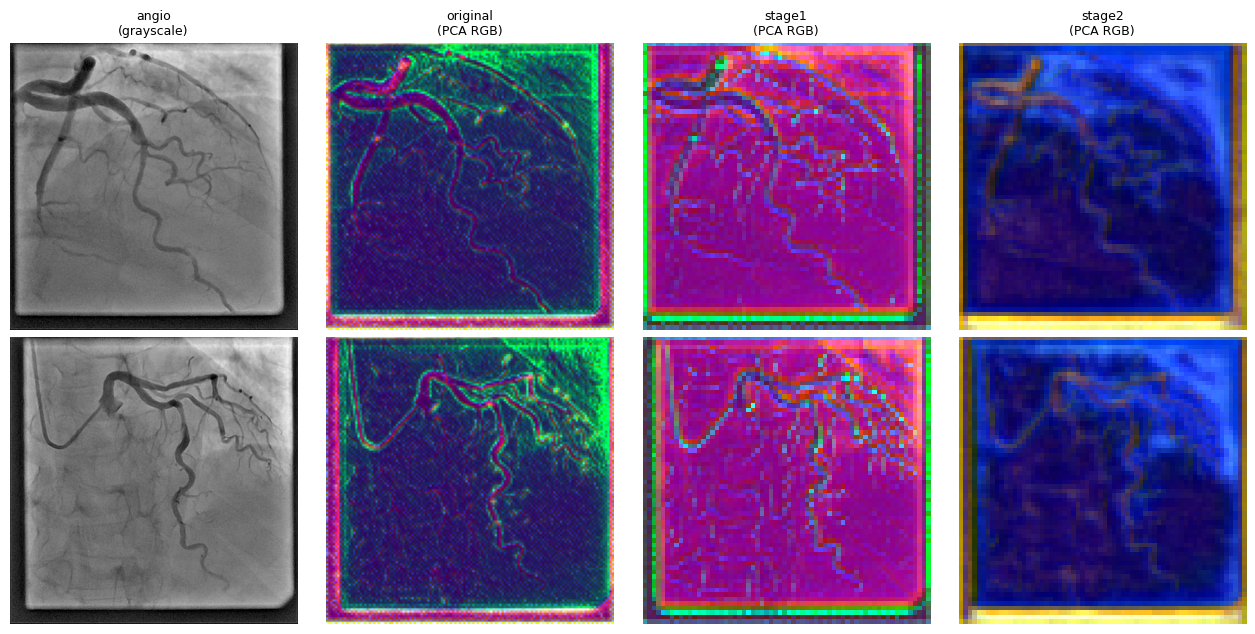
\includegraphics[width=\columnwidth]{figures/yanic/pca.png}
    \caption{RGB PCA of intermediate features (before \texttt{conv\_out}) for 4 coronary angiographies. Columns: original, MedVAE, Stage 1, Stage 2.}
    \label{fig:pca}
\end{figure}



\newpage
\section{MedVAE as a Latent Representation for Coronary Segmentation}

La haute résolution des images médicales est nécessaire pour préserver les détails diagnostiques, mais elle alourdit fortement le coût de calcul et de stockage des modèles d'apprentissage profond. Une réponse attractive consiste à compresser les images au moyen d'auto-encodeurs variationnels (VAE) \cite{kingma2014vae} génériques pré-entraînés à grande échelle. MedVAE \cite{varma2025medvaeefficientautomatedinterpretation}, entraîné sur plus d'un million d'images médicales, illustre cette approche : il réduit une image d'un facteur 16 (une réduction de 4 par dimension spatiale, soit une image $512 \times 512$ ramenée à un latent $128 \times 128$ à un seul canal) tout en cherchant à conserver les caractéristiques cliniquement pertinentes.

Cette compression reste toutefois intrinsèquement destructrice, et rien ne garantit qu'elle préserve l'information utile à toutes les tâches en aval. Les bénéfices de MedVAE ont été établis principalement sur des tâches de classification et de détection, qui reposent sur des caractéristiques globales. La segmentation fine d'artères coronaires constitue au contraire un cas défavorable. En effet, les structures à délimiter sont minces, tubulaires et peu contrastées, le nombre de classes est élevé (26 classes, à savoir le fond et 25 segments artériels) et leur distribution est fortement déséquilibrée. La question centrale que nous posons est donc la suivante : \textbf{une compression médicale avec perte préserve-t-elle suffisamment d'information anatomique pour permettre une segmentation coronarienne multi-classes ? À cette question s'en ajoute une seconde, d'ordre méthodologique : à quel endroit de la chaîne de traitement la compression doit-elle être intégrée pour que cette information demeure exploitable ?}

Pour y répondre, nous évaluons sur le jeu de données public ARCADE \cite{popov2024arcade} dans quelle mesure MedVAE peut servir de représentation intermédiaire pour la segmentation. Nous comparons trois stratégies tenant compte de la compression à une référence en pleine résolution, à savoir un U-Net \cite{ronneberger2015unet} entraîné sur les images originales : (i) segmenter directement à partir de la représentation latente compressée au moyen d'une tête de segmentation légère, (ii) adapter au préalable le compresseur au domaine coronarien par fine-tuning avant de segmenter depuis le latent, et (iii) entraîner un modèle de segmentation sur les images décompressées. Ces trois stratégies couvrent à la fois l'usage du latent et celui de l'espace pixel reconstruit, avec et sans adaptation au domaine. Nos résultats montrent que la segmentation directe depuis le latent à un seul canal échoue, que le fine-tuning orienté reconstruction ne suffit pas à rendre ce latent exploitable, mais que l'espace pixel décompressé préserve les structures coronaires et procure même un léger gain, concentré sur les classes les plus difficiles, par rapport à la référence.

\subsection{Méthodes}

\paragraph{Données et prétraitement.}
Nous utilisons le jeu de données public ARCADE \cite{popov2024arcade} (1\,200 angiographies en niveaux de gris, $512 \times 512$), dont les annotations COCO sont converties en masques denses à 26 classes. Nous adoptons une partition 80\,\%/20\,\% pour l'entraînement et la validation, et reportons toutes les performances sur le jeu de test officiel de 300 images. Les intensités sont normalisées dans $[0,1]$ et l'entraînement emploie une augmentation classique (retournements, transformations affines, ajustements de contraste et de luminosité, bruit gaussien, CLAHE) via Albumentations \cite{buslaev2020albumentations}. Les transformations géométriques sont appliquées conjointement à l'image et à son masque, afin de préserver leur alignement.

\paragraph{Compresseur MedVAE.}
Le compresseur est la variante \texttt{medvae\_4\_1\_2d} de MedVAE \cite{varma2025medvaeefficientautomatedinterpretation}, qui réduit chaque dimension spatiale d'un facteur 4 : une image $512 \times 512$ est encodée en un latent $128 \times 128$ à un seul canal, soit une réduction d'un facteur 16 en surface. Sauf indication contraire, ses poids sont gelés.

\paragraph{Conditions expérimentales.}
Nous comparons trois stratégies tenant compte de la compression à une référence en pleine résolution, ainsi qu'un contrôle diagnostique. Chaque condition est illustrée par son schéma de traitement.

\textbf{A (référence).} Un U-Net \cite{ronneberger2015unet} à encodeur ResNet-34 \cite{he2016resnet} pré-entraîné sur ImageNet, entraîné de bout en bout sur les images originales (Fig.~\ref{fig:pipe_a}).
\begin{figure}[H]
\centering
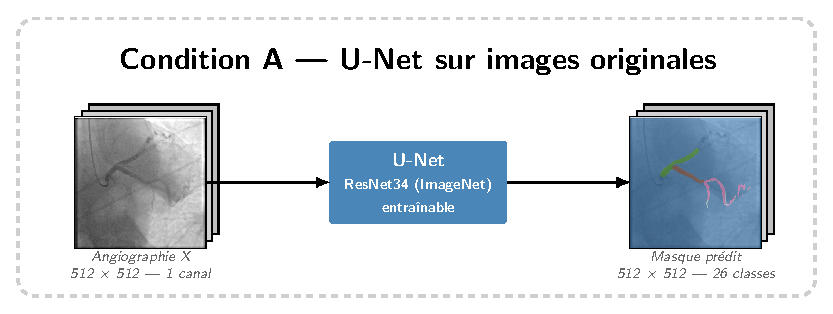
\includegraphics[width=\columnwidth]{figures/theo/cond_A2.pdf}
\caption{Condition A. Référence en pleine résolution : un U-Net segmente directement l'angiographie originale.}
\label{fig:pipe_a}
\end{figure}

\textbf{A$^{*}$ (contrôle hors distribution).} Le U-Net de la condition A, sans aucun réentraînement, est appliqué à des images d'abord encodées puis décodées par MedVAE (Fig.~\ref{fig:pipe_astar}). Cette condition isole l'effet brut de la compression en espace pixel sur un modèle non adapté, indépendamment de tout apprentissage.
\begin{figure}[H]
\centering
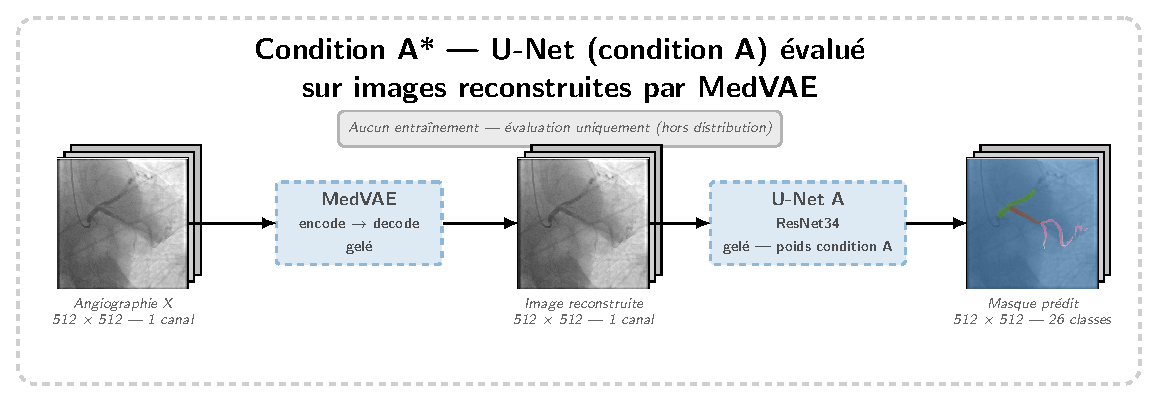
\includegraphics[width=\columnwidth]{figures/theo/cond_Astar.pdf}
\caption{Condition A$^{*}$. Le U-Net gelé de A est évalué sur des images reconstruites par MedVAE, sans réentraînement.}
\label{fig:pipe_astar}
\end{figure}

\textbf{B (segmentation depuis le latent).} Le latent $128 \times 128 \times 1$ produit par l'encodeur MedVAE gelé alimente une tête de segmentation légère (Fig.~\ref{fig:pipe_b}) : une projection $1 \times 1$ vers 128 canaux, deux blocs convolutifs entrecoupés de sur-échantillonnages bilinéaires pour revenir à $512 \times 512$, et une classification finale en 26 classes.
\begin{figure}[H]
\centering
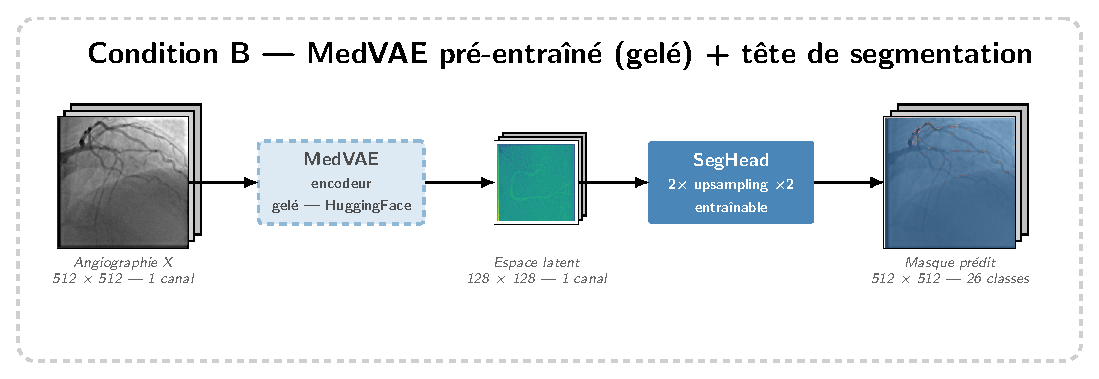
\includegraphics[width=\columnwidth]{figures/theo/cond_B.pdf}
\caption{Condition B. Une tête légère segmente directement le latent compressé à un seul canal de l'encodeur MedVAE pré-entraîné gelé.}
\label{fig:pipe_b}
\end{figure}

\textbf{C (fine-tuning de domaine).} Identique à B, mais l'encodeur MedVAE est d'abord fine-tuné sur ARCADE par une perte de reconstruction avant d'être gelé (Fig.~\ref{fig:pipe_c}), afin de tester si l'adaptation au domaine coronarien enrichit le latent.
\begin{figure}[H]
\centering
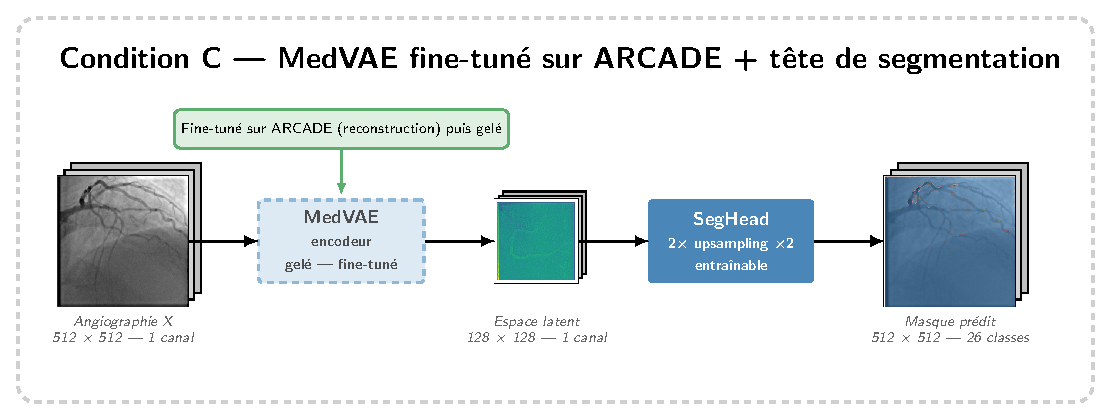
\includegraphics[width=\columnwidth]{figures/theo/cond_C.pdf}
\caption{Condition C. Comme B, l'encodeur MedVAE étant au préalable fine-tuné sur ARCADE puis gelé.}
\label{fig:pipe_c}
\end{figure}

\textbf{D (segmentation des images reconstruites).} Un U-Net identique à A est entraîné non pas sur les images originales mais sur leur version reconstruite par MedVAE (Fig.~\ref{fig:pipe_d}). Contrairement à A$^{*}$, le réseau s'adapte ici aux artefacts de la compression.
\begin{figure}[H]
\centering
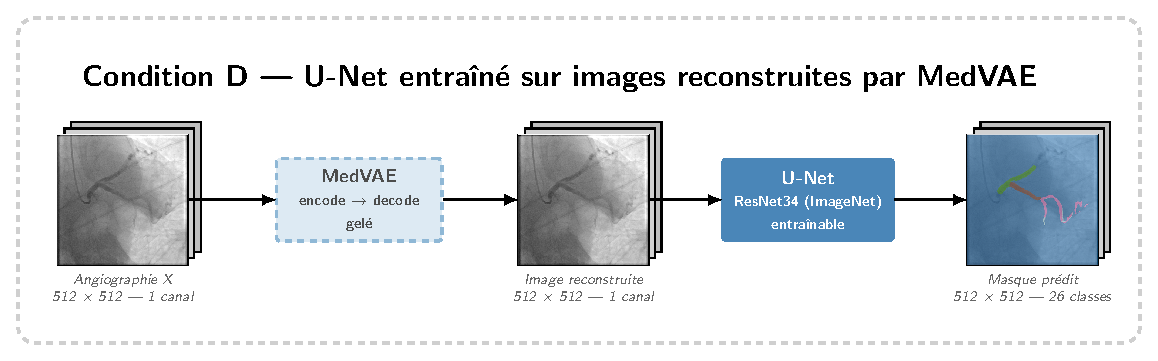
\includegraphics[width=\columnwidth]{figures/theo/cond_D.pdf}
\caption{Condition D. Le U-Net est réentraîné sur les images reconstruites par MedVAE, ce qui l'adapte aux artefacts de compression.}
\label{fig:pipe_d}
\end{figure}

\paragraph{Entraînement et évaluation.}
Tous les modèles minimisent une perte composite combinant à parts égales une perte de Dice et une entropie croisée :
\begin{equation}
\mathcal{L} = 0{,}5\,\mathcal{L}_{\text{Dice}} + 0{,}5\,\mathcal{L}_{\text{CE}}.
\end{equation}
Ce choix répond directement au déséquilibre massif des classes. La perte de Dice \cite{milletari2016vnet} mesure le recouvrement entre prédiction et vérité terrain indépendamment de la taille des régions, ce qui empêche le fond majoritaire de dominer l'optimisation. L'entropie croisée, calculée pixel à pixel, fournit quant à elle un gradient plus stable, en particulier en début d'entraînement. L'optimisation emploie AdamW, un ordonnancement cosinus du taux d'apprentissage et la précision mixte, avec arrêt précoce sur le Dice de validation. Les performances sont rapportées par le coefficient de Dice et l'IoU, moyennés sur les 26 classes.

\subsection{Résultats}

Le tableau~\ref{tab:results} résume les performances sur le test, et la figure~\ref{fig:val_curves} les dynamiques d'entraînement. Des exemples de prédictions qualitatives pour chaque condition sont reportés en annexe (figures~\ref{fig:pred_a} à~\ref{fig:pred_d}).

\begin{table}[H]
\caption{Performances sur le test ARCADE (300 images), moyennées sur les 26 classes.}
\centering
\begin{tabular}{llcc}
\toprule
Cond. & Modèle entraîné sur & Dice & IoU \\
\midrule
A        & Images originales (pixel)            & 0,433 & 0,499 \\
A$^{*}$  & Images reconstruites (éval. seule)   & 0,434 & 0,497 \\
B        & Latent pré-entraîné                  & 0,038 & 0,005 \\
C        & Latent fine-tuné                     & 0,039 & 0,000 \\
D        & Images reconstruites (pixel)         & \textbf{0,451} & 0,495 \\
\bottomrule
\end{tabular}
\label{tab:results}
\end{table}

\begin{figure}[t]
\centering
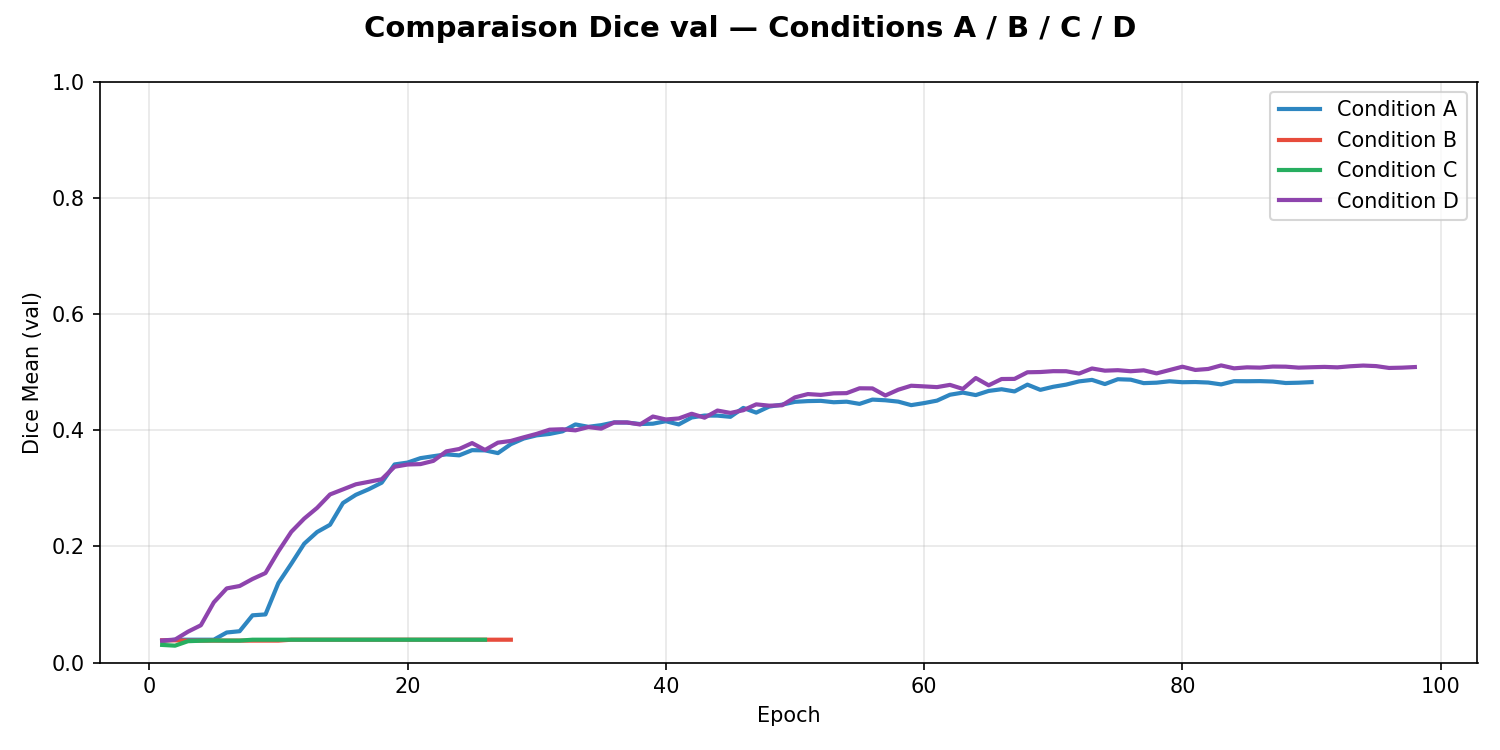
\includegraphics[width=\columnwidth]{figures/theo/comparaison_conditions.png}
\caption{Dice de validation au cours de l'entraînement. Les conditions A et D convergent vers un Dice d'environ 0,50, D dépassant légèrement A en fin de course. Les conditions B et C, qui segmentent depuis le latent compressé, restent bloquées autour de 0,04 dès les premières epochs et déclenchent un arrêt précoce avant l'epoch 30 : la tête n'apprend jamais, que le compresseur soit pré-entraîné (B) ou fine-tuné sur le domaine (C).}
\label{fig:val_curves}
\end{figure}

\begin{figure*}[t]
\centering

\includegraphics[width=\textwidth]{figures/theo/dice_per_class.png}
\caption{Dice par classe sur le test (C0 = fond, C1 à C25 = segments coronariens). Les conditions A, A$^{*}$ et D segmentent correctement les segments fréquents et épais (C1 à C7) tandis que B et C ne prédisent que le fond. Le gain de D sur A se concentre sur les segments rares et fins que A n'apprend pas (par exemple C11, C18, C19), alors que A et A$^{*}$ sont quasi indiscernables, ce qui confirme que la compression en espace pixel ne dégrade pas la segmentation.}
\label{fig:dice_class}
\end{figure*}

\paragraph{La segmentation depuis le latent échoue.}
Les conditions B et C s'effondrent à un Dice de 0,038 et 0,039, contre 0,433 pour la référence A ; la figure~\ref{fig:dice_class} montre que seul le fond (C0) est correctement prédit, aucun segment artériel n'étant appris ; les prédictions sont presque entièrement assignées au fond (figures~\ref{fig:pred_b} et~\ref{fig:pred_c}). Cet effondrement résulte de la conjonction de deux facteurs. D'une part, le déséquilibre des classes est extrême : le fond représente près de 95\,\% des pixels. Bien que la perte composite (Dice et entropie croisée) soit en partie destinée à contrer ce déséquilibre, la solution triviale consistant à tout prédire comme fond demeure un minimum local fortement attracteur dès lors que le modèle ne reçoit pas un signal d'entrée suffisamment riche ; B et C l'atteignent dès les premières epochs et ne le quittent jamais (figure~\ref{fig:val_curves}). D'autre part, la tête de segmentation opère sur un latent à un seul canal et ne dispose d'aucune représentation multi-échelles : contrairement au U-Net, elle n'a ni connexions de saut ni hiérarchie de résolutions susceptibles de fournir le signal spatial fin nécessaire à la localisation de structures tubulaires minces. Ces deux facteurs se renforcent : faute de signal exploitable, la tête ne dispose d'aucun gradient utile pour s'extraire du minimum trivial. Le fine-tuning du compresseur (C) n'y change rien : optimiser MedVAE pour la reconstruction améliore la fidélité visuelle des images mais n'enrichit pas le pouvoir discriminant du latent pour la segmentation. L'IoU de C tombe d'ailleurs à 0,000, le modèle ne prédisant que le fond : l'intersection avec la vérité terrain est nulle pour chacune des 25 classes d'artères, ce qui annule l'IoU moyen sur ces classes.

\paragraph{La compression en espace pixel est neutre.}
La condition A$^{*}$ sert de contrôle : en appliquant le modèle de référence, sans réentraînement, à des images reconstruites par MedVAE, elle mesure l'effet de la seule compression, indépendamment de toute adaptation du réseau. Son Dice de 0,434 est quasi identique à celui de la référence A (0,433), et la figure~\ref{fig:dice_class} montre une correspondance classe par classe quasi parfaite, les prédictions de A et A$^{*}$ étant visuellement identiques (figures~\ref{fig:pred_a} et~\ref{fig:pred_astar}). La compression 16× préserve donc l'information anatomique exploitée par le réseau lorsqu'elle est rendue en espace pixel, au point qu'un modèle non adapté n'en souffre pas.

\paragraph{S'adapter à la reconstruction apporte un gain ciblé.}
La condition D obtient le meilleur Dice (0,451). Cette amélioration du Dice s'accompagne d'un IoU légèrement inférieur à A (0,495 contre 0,499), cohérent avec les occasionnelles sur-segmentations observées en annexe : D capture davantage de vrais positifs sur les segments rares, au prix d'un excès de faux positifs sur certains cas. L'apport propre de l'adaptation à la compression se lit le plus proprement dans l'écart entre D et A$^{*}$ : ces deux conditions traitent exactement la même entrée, à savoir des images reconstruites par MedVAE, et ne diffèrent que par un point, le réseau de D ayant été réentraîné sur ces images quand celui de A$^{*}$ ne l'a pas été. Leur écart, $\Delta = 0{,}451 - 0{,}434 = +0{,}017$, mesure donc le bénéfice de la seule adaptation aux artefacts de compression, sans le confondre avec l'effet de la compression elle-même (qui est nul, A$^{*}$ $\approx$ A). Ce gain, réel mais modeste, est entièrement concentré sur les segments rares et fins que la référence ne parvenait pas à apprendre : C11 passe de 0,000 à 0,126, C18 de 0,031 à 0,113 et C19 de 0,015 à 0,191, tandis que D perd légèrement sur les grands segments (C1 : 0,789 à 0,753). Ces branches fines, absentes des prédictions de A, réapparaissent dans celles de D (figure~\ref{fig:pred_d}). Nous interprétons cet effet comme une régularisation : la reconstruction MedVAE agirait comme un débruitage qui, en atténuant la variabilité d'acquisition haute fréquence, faciliterait l'apprentissage des structures fines. Nos expériences ne permettent toutefois pas d'établir ce mécanisme directement, et cette interprétation demande à être confirmée.

\subsection{Discussion}

Nos expériences répondent aux deux volets de la problématique. Sur la préservation de l'information, une compression médicale avec perte de facteur 16 conserve assez d'information anatomique pour la segmentation coronarienne multi-classes, à condition de l'exploiter en espace pixel : la dégradation est nulle (A$^{*}$ $\approx$ A) et l'adaptation à la compression apporte même un gain propre, mesuré sans confusion par l'écart contrôlé D contre A$^{*}$ ($+0{,}017$), concentré sur les segments les plus difficiles. Sur le point d'intégration, le latent à un seul canal de MedVAE est en revanche inadapté à une tâche dense et fine : la segmentation directe depuis le latent échoue, et le fine-tuning orienté reconstruction ne la débloque pas.

La principale limite tient à la variante de compression étudiée. Un latent à plusieurs canaux, ou l'exploitation des cartes intermédiaires de l'encodeur plutôt que du seul goulot d'étranglement, pourrait restaurer l'information perdue ; de même, un fine-tuning supervisé par un objectif de segmentation, plutôt que de reconstruction, est une piste naturelle. Nos résultats délimitent ainsi clairement le régime dans lequel un compresseur médical générique est utile pour la segmentation : non comme un espace latent à segmenter directement, mais comme un préprocesseur en espace pixel dont le débruitage profite aux structures les plus difficiles.


\section{Conclusion}



\newpage
\balance
\bibliographystyle{plain}
\bibliography{references}

\newpage 
\appendix
\section{Prédictions qualitatives}

\begin{figure}[H]
\centering

\includegraphics[width=\columnwidth]{figures/theo/predictions_condition_a_unet.png}
\caption{Condition A (U-Net de référence sur images originales). De gauche à droite : image d'entrée, vérité terrain, prédiction ; quatre cas de test. Les segments principaux sont bien délimités, mais les branches fines et les segments rares sont fréquemment omis.}
\label{fig:pred_a}
\end{figure}

\begin{figure}[H]
\centering
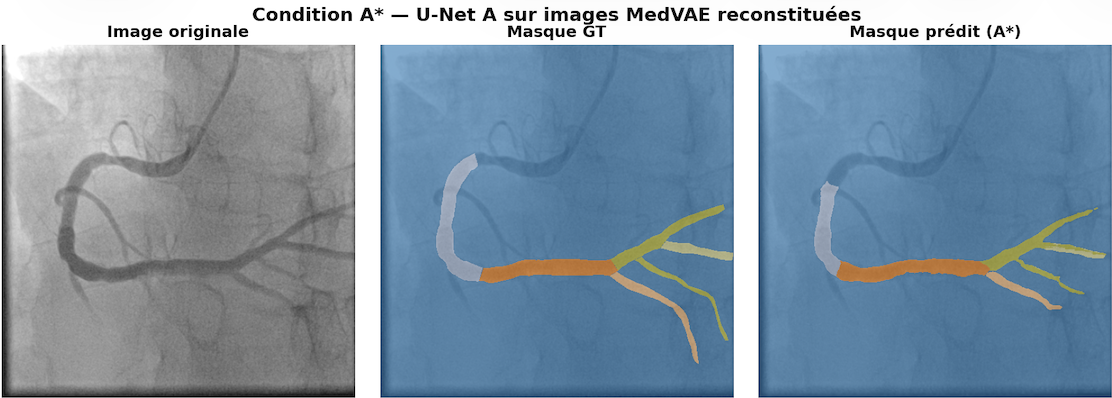
\includegraphics[width=\columnwidth]{figures/theo/predAstar.png}
\caption{Condition A$^{*}$ (U-Net de A appliqué sans réentraînement à des images reconstruites par MedVAE), un exemple représentatif. La prédiction est visuellement identique à celle de A, illustrant que la compression 16× en espace pixel préserve l'information exploitée par le réseau.}
\label{fig:pred_astar}
\end{figure}

\begin{figure}[H]
\centering
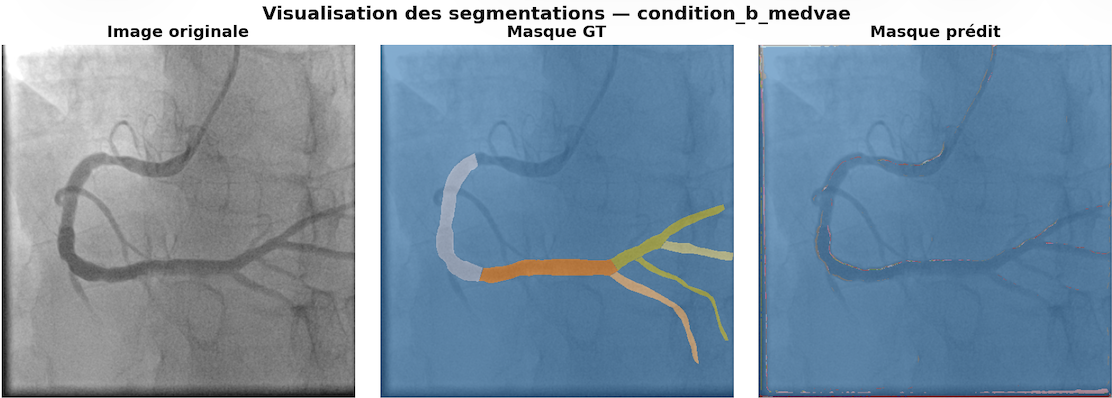
\includegraphics[width=\columnwidth]{figures/theo/predB.png}
\caption{Condition B (segmentation depuis le latent MedVAE pré-entraîné via une tête légère), un exemple représentatif. La prédiction est presque entièrement assignée au fond : le latent à un seul canal ne porte pas l'information nécessaire pour discriminer les segments.}
\label{fig:pred_b}
\end{figure}

\begin{figure}[H]
\centering
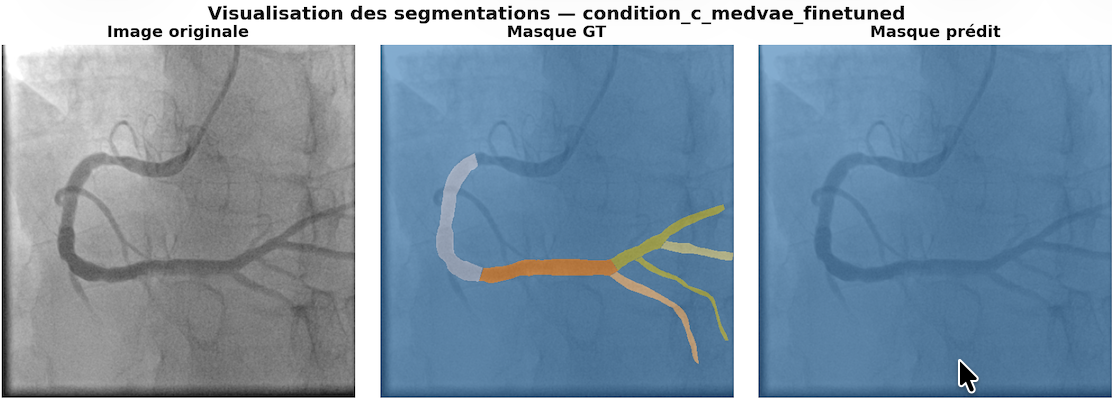
\includegraphics[width=\columnwidth]{figures/theo/predC.png}
\caption{Condition C (identique à B, compresseur fine-tuné sur ARCADE), un exemple représentatif. L'adaptation au domaine n'apporte aucune amélioration visible ; la prédiction reste dominée par le fond.}
\label{fig:pred_c}
\end{figure}

\begin{figure}[H]
\centering
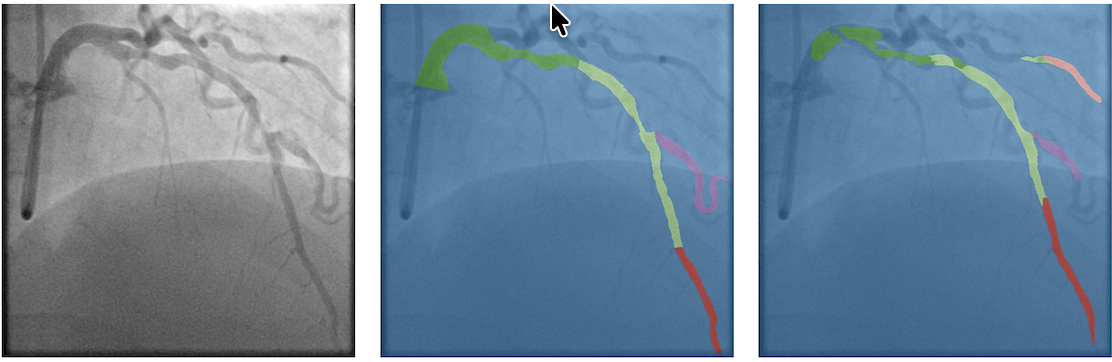
\includegraphics[width=\columnwidth]{figures/theo/conDmieux.png}
\caption{Condition D (U-Net réentraîné sur images reconstruites par MedVAE), un exemple représentatif. La délimitation des segments épais reste comparable à A et plusieurs branches fines absentes de A sont ici récupérées, au prix d'occasionnelles sur-segmentations.}
\label{fig:pred_d}
\end{figure}

% ------------------------------------------------------------
\newpage
\section{PSNR masqué sur les vaisseaux : détail}
\label{app:mpsnr}

Le PSNR masqué ($\mathrm{mPSNR}$) restreint le calcul de l'erreur aux seuls vaisseaux afin d'écarter le biais du fond, largement majoritaire et cliniquement non pertinent. Les annotations polygonales d'ARCADE sont rastérisées en masque binaire (\texttt{cv2.fillPoly}), puis redimensionnées par interpolation au plus proche voisin pour préserver leur binarité. L'erreur quadratique moyenne n'est évaluée que sur cet ensemble de pixels, noté $\mathcal{M}$ :
\begin{equation}
\mathrm{mPSNR}(x, y) = 10\,\log_{10}\!\frac{D^2}
{\frac{1}{|\mathcal{M}|}\sum_{p \in \mathcal{M}} \big(x_p - y_p\big)^2},
\label{eq:mpsnr}
\end{equation}
où $D$ est la dynamique des intensités ($D = 1$ pour des images normalisées dans $[0,1]$).

% ---------- Figure : schéma du PSNR masqué ----------
\begin{figure}[h]
  \centering
  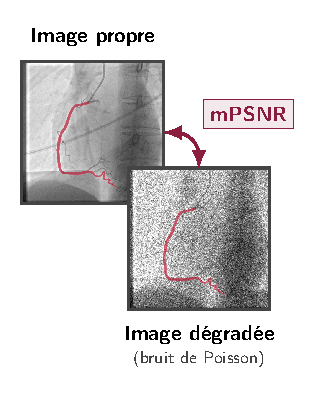
\includegraphics[width=0.65\linewidth]{figures/elias/mpsnr.pdf}
  \caption{Principe du PSNR masqué sur un exemple réel d'ARCADE. L'image
  propre et sa version dégradée partagent le même masque de vaisseaux $\mathcal{M}$
  (rouge). L'erreur n'est évaluée que sur ces pixels ($\approx 2\%$ de la surface).}
  \label{fig:masked-psnr}
\end{figure}


% ------------------------------------------------------------
\newpage
\section{Visualisation des dégradations synthétiques}
\label{app:degradations}

% ---------- Figure pleine largeur : grille de dégradations ----------
\begin{figure*}[h]
  \centering
  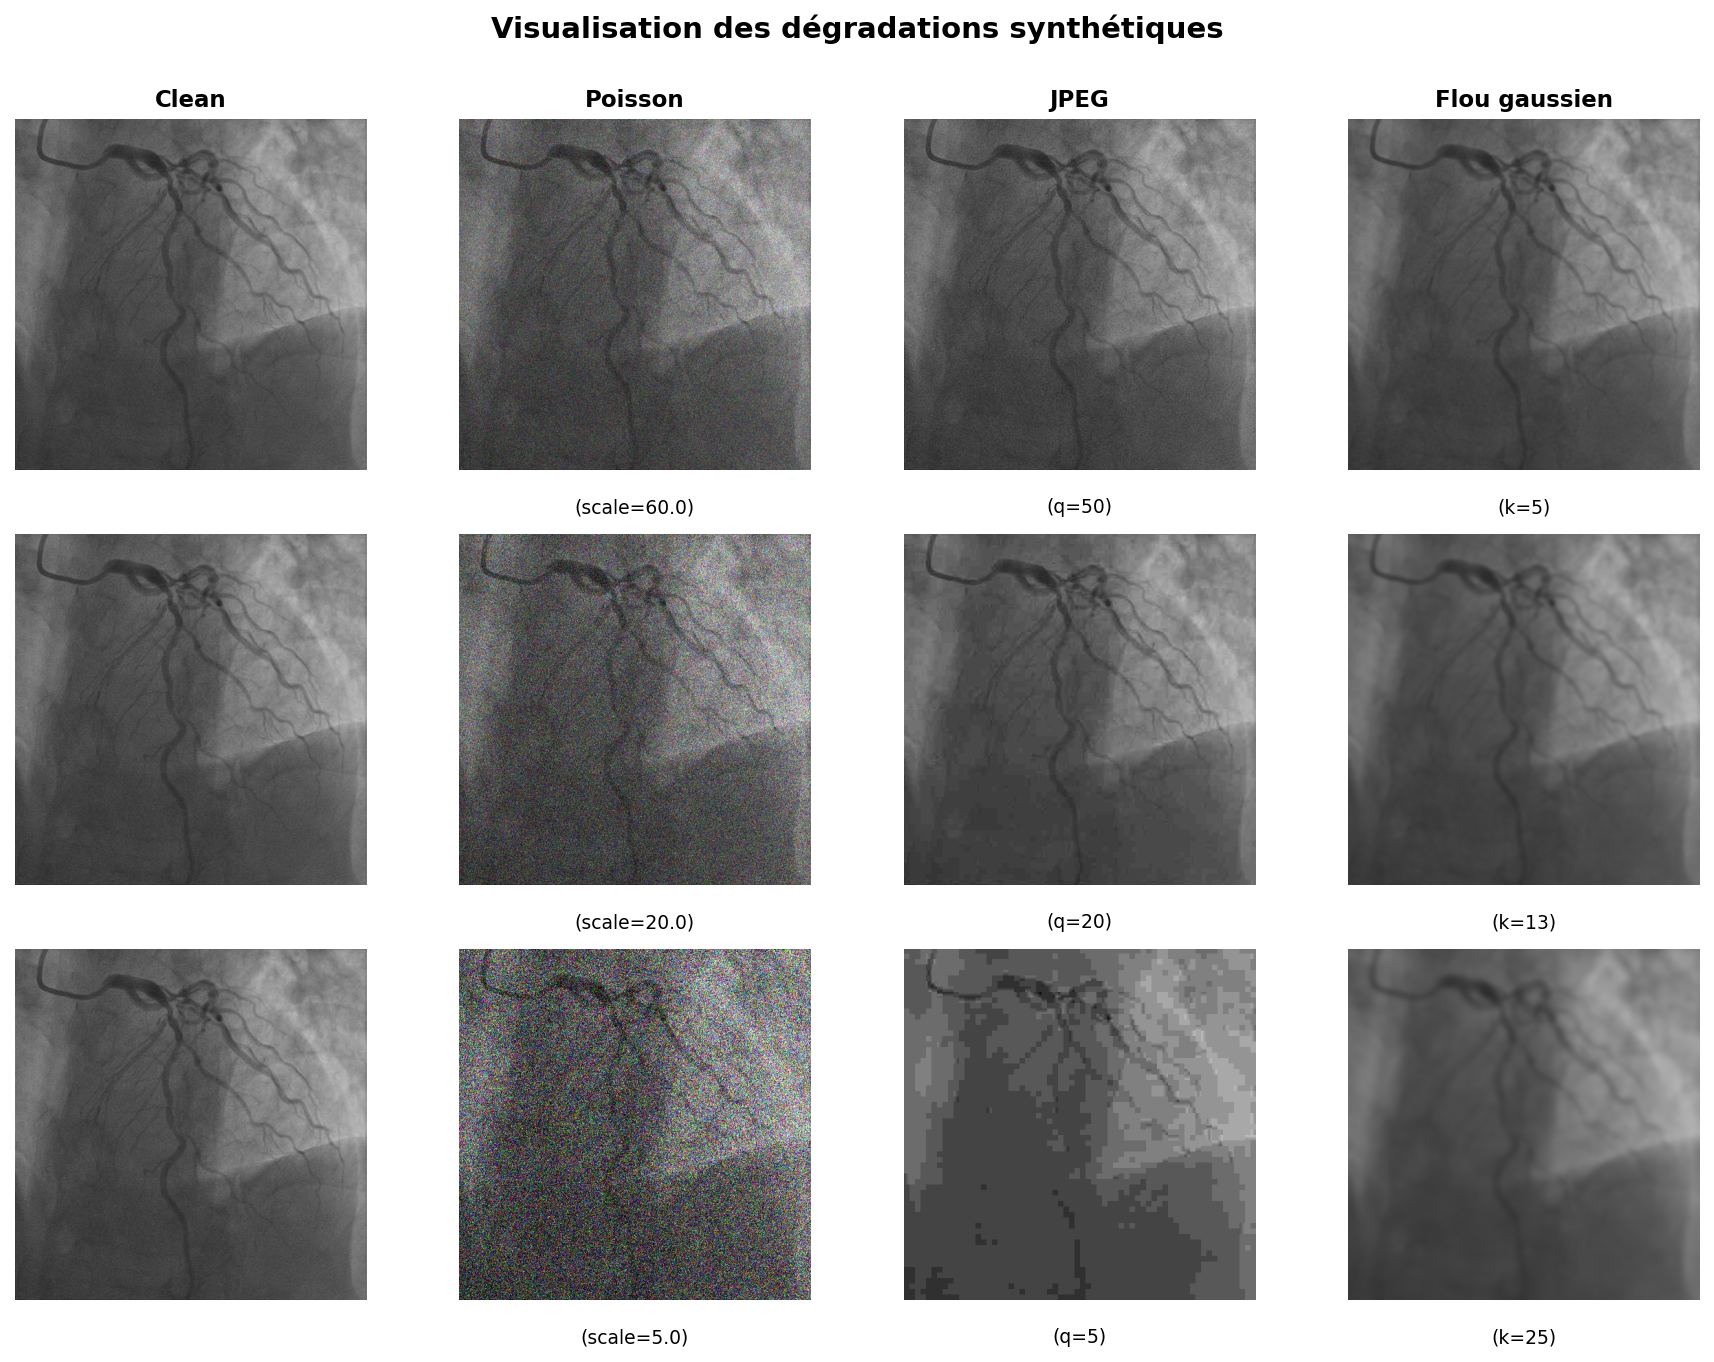
\includegraphics[width=0.95\textwidth]{figures/elias/degradation_visual.png}
  \caption{Visualisation des dégradations synthétiques appliquées en entrée (détail). De gauche à droite : image propre (\emph{Clean}), bruit de Poisson, compression JPEG, flou gaussien. L'intensité de la dégradation augmente de haut en bas, faisant apparaître l'injection de hautes fréquences (bruit, blocs $8\times8$) ou au contraire leur suppression (lissage passe-bas).}
  \label{fig:degradation-visual}
\end{figure*}

\end{document}
